
\chapter{Results}
\section{Simulation of Capacitance values}
\subsection{Comparision of Capacitance in the simulation with a sphere geometry}
The simulation of the capacitance for the cylindric geometry as a function of different distances with COMSOL leads to the following figure.The simulation of two spheres as well as the approximation formula result in a general shift which is due to the fact that it is a three electrode arrangement as the wall of the low-voltage introduces a new capacitance between the upper electrode and the wall which is not affected by the distance variation. This results in a reduction of the capacitance compared to the two spheres geometry. Thus, the simulated values for the low voltage test cell seem reasonable if one compares them to the results of the capacitance between two spheres. \newline 



\begin{figure}[]
	\centering
	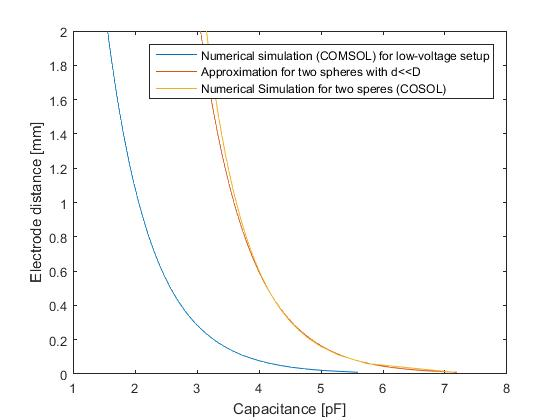
\includegraphics[scale=1]{figures/Comparison_Low_voltage_Two_spheres}		
	\caption[Kurze Abbildungsbeschreibung]{Dependency of the electrode distance on the capacitance for the low voltage setup and two spheres $\epsilon = 3.5$ } 
	\label{fig.waveforms}
\end{figure}

\section{Complex effective permittivity}
\subsection{}

\chapter{Results}
\section{Simulation of Capacitance values}
\subsection{Comparision of Capacitance in the simulation with a sphere geometry}
The simulation of the capacitance for the cylindric geometry as a function of different distances with COMSOL leads to the following figure.The simulation of two spheres as well as the approximation formula result in a general shift which is due to the fact that it is a three electrode arrangement as the wall of the low-voltage introduces a new capacitance between the upper electrode and the wall which is not affected by the distance variation. This results in a reduction of the capacitance compared to the two spheres geometry. Thus, the simulated values for the low voltage test cell seem reasonable if one compares them to the results of the capacitance between two spheres. \newline 


\begin{figure}[htbp]
	\centering
	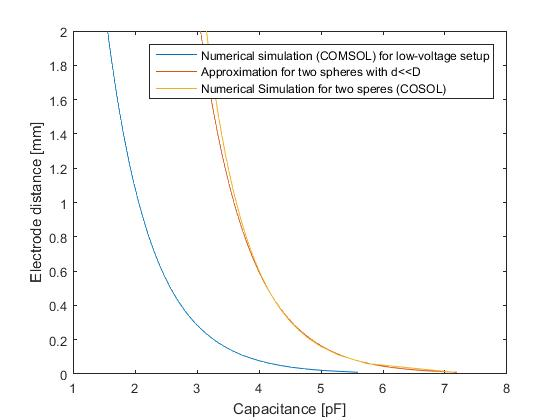
\includegraphics[scale=0.3]{figures/Comparison_Low_voltage_Two_spheres}		


	\caption[Kurze Abbildungsbeschreibung]{Dependency of the electrode distance on the capacitance for the low voltage setup and two spheres $\epsilon = 3.5$ }%

	\label{fig.waveforms}
\end{figure}

\section{Complex effective permittivity}
\subsection{}

\section{Performance of integrator}

\section{Dielectric Spectroscopy}

\begin{figure}[htbp]
\centering
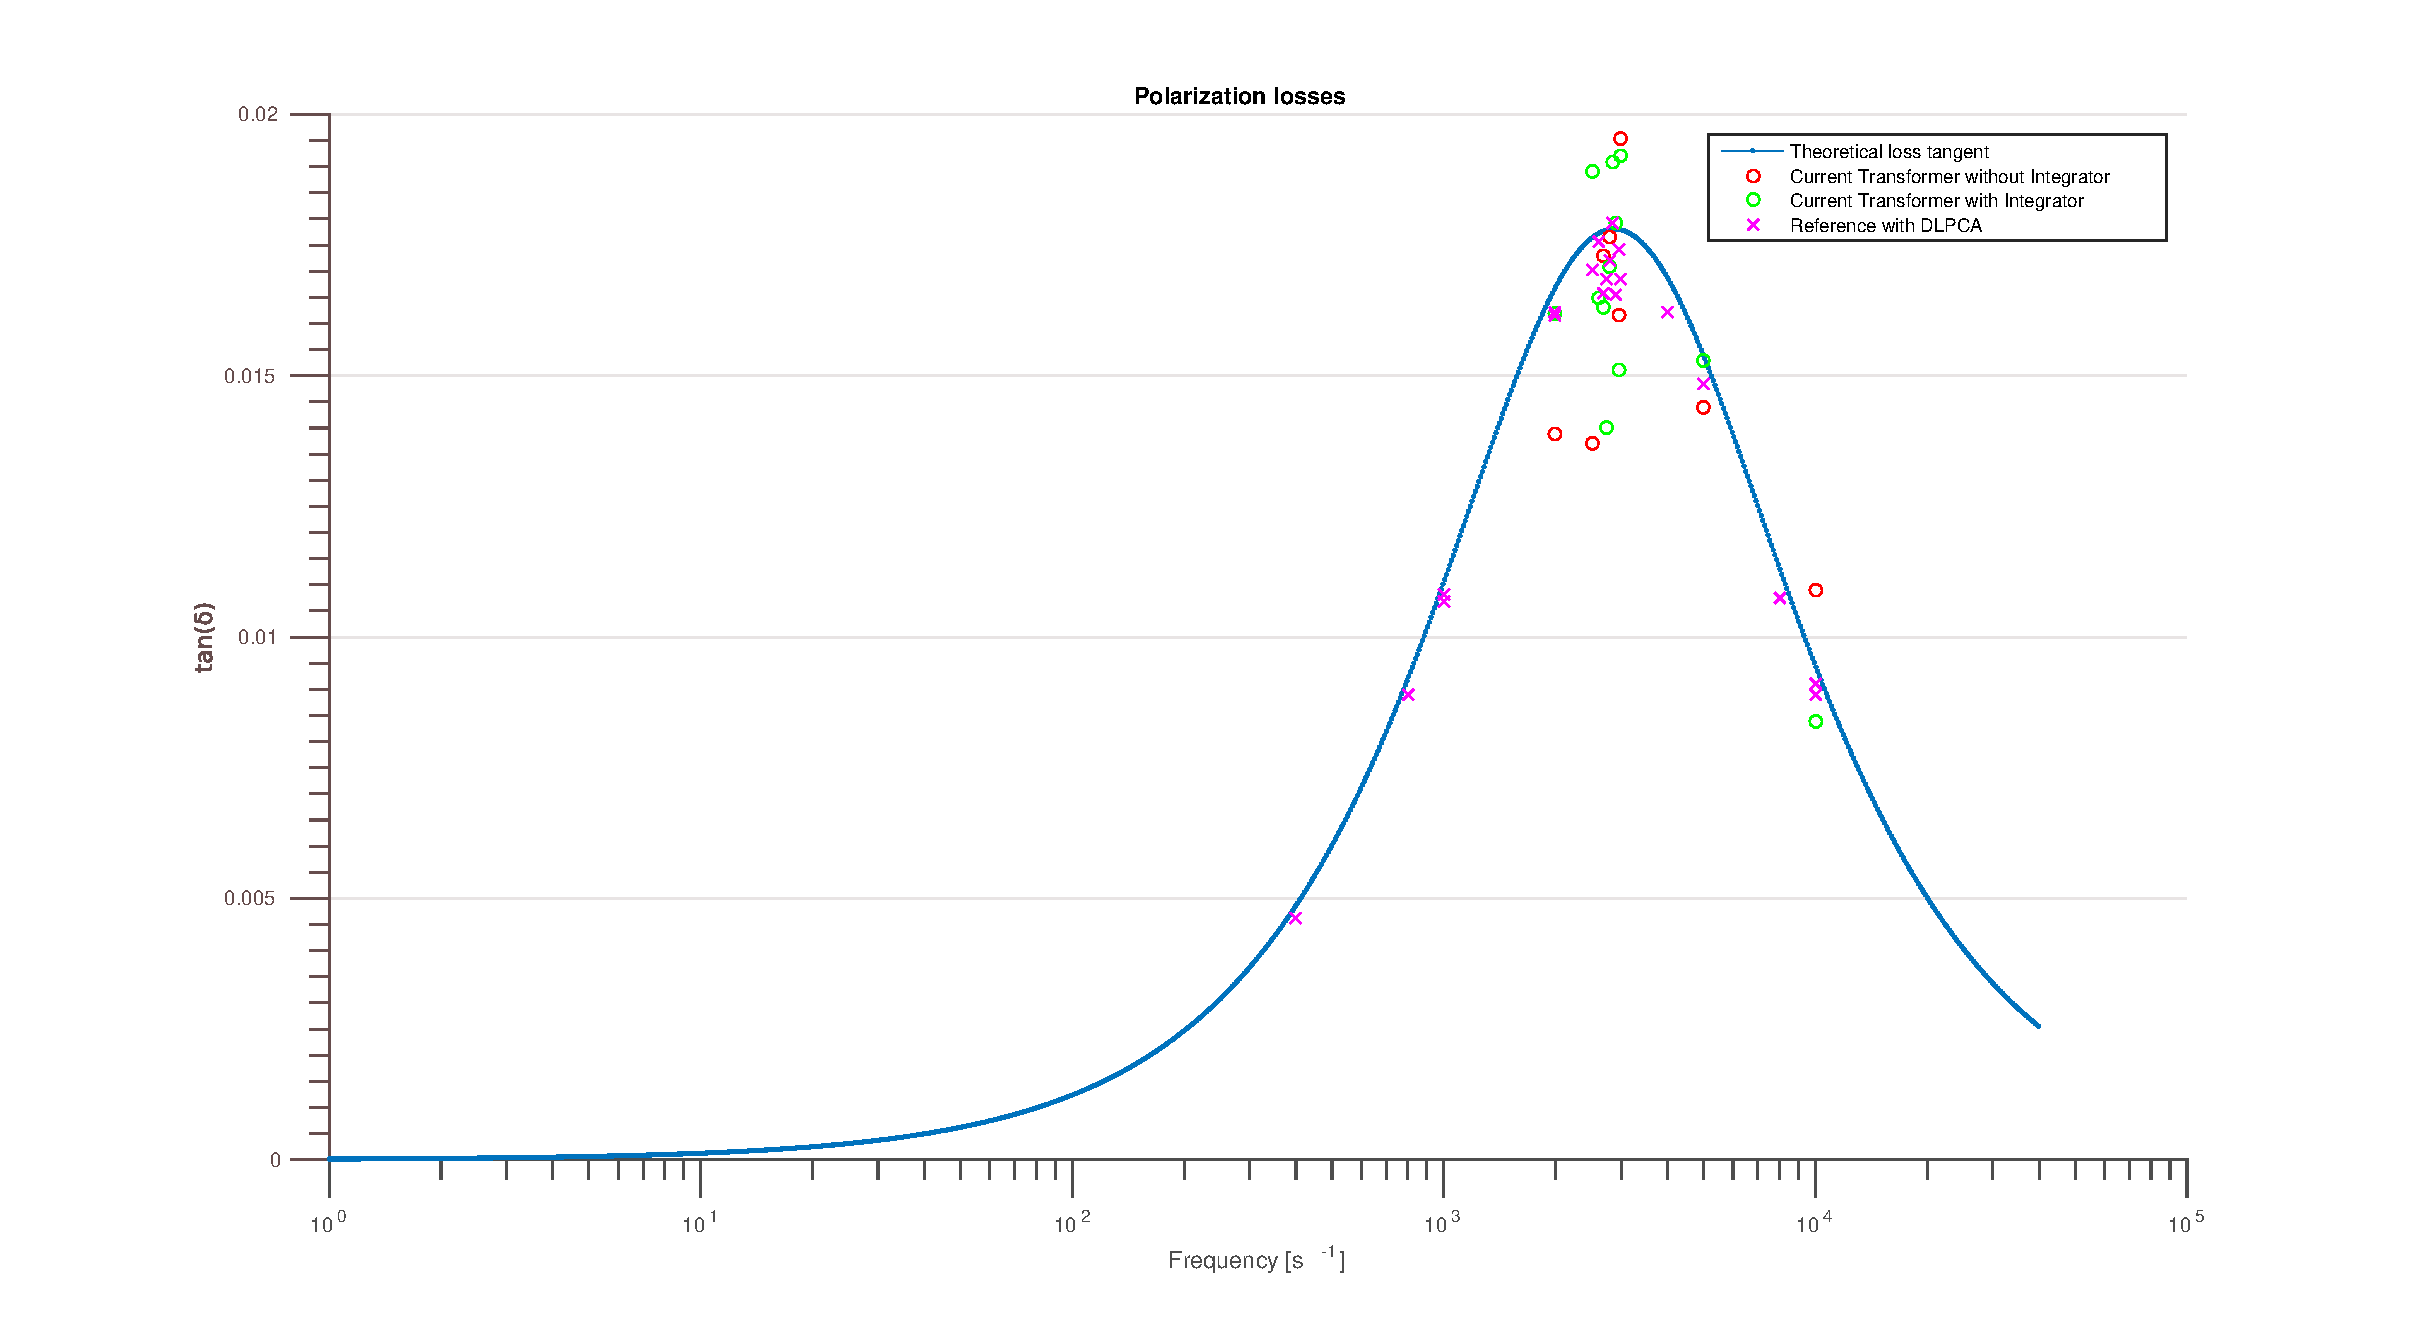
\includegraphics[scale=0.3]{figures/Results/Spectroscopy/spectroscopywithoutbars}
\caption[Kurze Abbildungsbeschreibung]{Measurements of dielectric loss tangent in different setup configurations}

\label{fig.spectroscopy}

\end{figure}
The three data series created from the spectroscopy experiment using the Debye model are shown in the graph above. The solid blue line represents the theoretical  dielectric loss tangent given the parameters of the components in the debye model
as a function of the frequency.
The components were assumed to be ideal and not to be temperature dependent.
The magenta data points can be used as a reference to evaluate the performance of the current transformer as these measurement points
were obtained with a industry standard low-noise current amplifier (DLPCA). 
The red points were recieved by replacing the DLPCA with the current transformer.
The green points were measured with the integrator in place, effectively integrating the voltage signal generated by the current transformer.
\newpage
\begin{figure}[htbp]
 \centering
 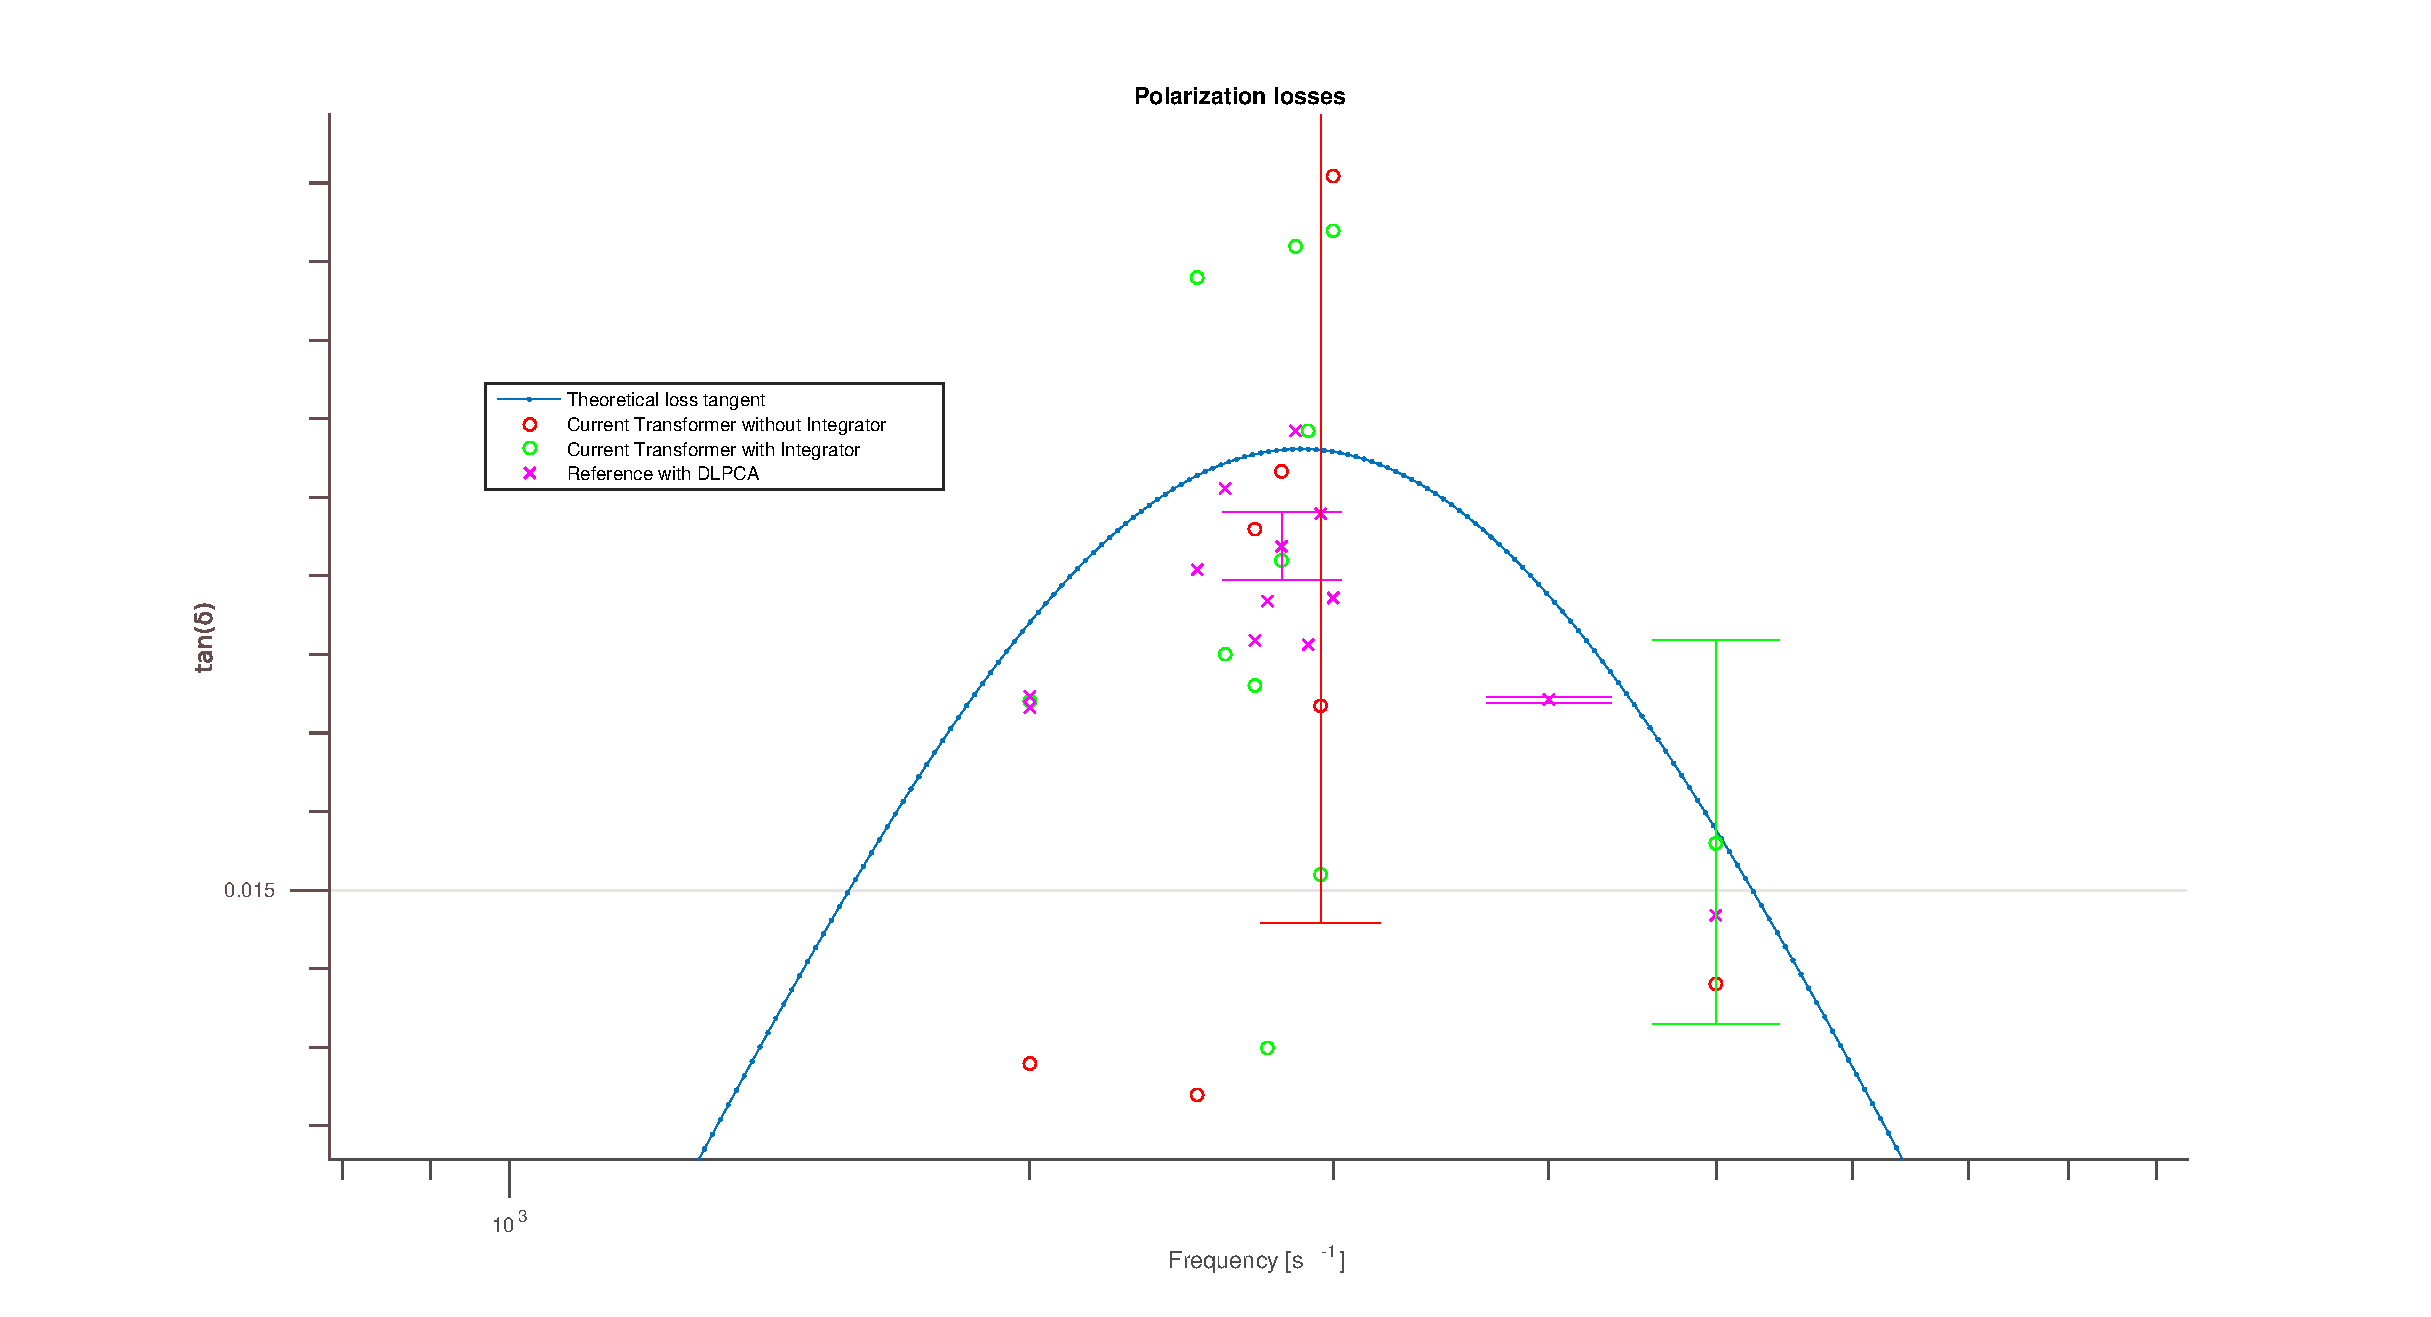
\includegraphics[scale=0.3]{figures/Results/Spectroscopy/errorbarsbettercolor}

\caption[Kurze Abbildungsbeschreibung]{Confidence intervals}
\label{fig.spectroscopy2}
\end{figure}

In order to adequately analyze the data points, the above graphic shows the previous plot
zoomed in around the maximum loss tangent since the deviation from the theoretical result seem to be the largest here.
The confidence intervals were added for a few points in each measurement series.

First it can be noted that while the reference measurements fit the curve the closest, the theoretical values are still not
within the measurements confidence intervals and the error can be greater than 10\%. To sum up the measurements conducted with
the current transformer, it can be stated that the measurement performance was significantly worse than the reference. Not only do they deviate further from the theoretical values
but they also have a larger variance. Which means that one cannot consistently predict a reasonable range for the mean of said measurement, at least not for only 9 phase averages.
While the use of the integrator succesfully lowered the deviation and shrinked the confidence intervals by a factor of 2 to 3, the measurement accuracy is still nowhere close to the one obtained with the DLPCA.

\subsection{Analysis of Noise Parameters}

In order to identify one of the sources to which the errors can be attributed, the noise level at the input and at the ouput was measured and analyzed to gain an estimation about how much noise was added in the system.
Using the current transformer in both configurations, i.e. with and without the integrator, the following parameters were measured. 

\newpage

\textit{Data without integrator:}
\begin{center}
\begin{tabular}{|m{3cm}|m{3cm}|m{1.3cm}|m{4cm}|m{2cm}|} 
\hline
frequency [Hz]& SNR$_{in}$ & SNR$_{out}$ & Noise Figure [dB] & Noise Floor \\ 
\hline \hline
2000 & 2.40E+07 & 16.31 & \cellcolor{blue!25}61.79 & 1.00E-05 \\ 
\hline
2500 & 1.8E+07 & 25.69 & \cellcolor{blue!25}58.55 & 1.00E-05 \\ 
\hline
2700 & 5.10E+07 & 31.02 & \cellcolor{blue!25}42.23 & 1.00E-05 \\ 
\hline
3000 & 5.13E+05 & 42.04 & \cellcolor{blue!25}40.86 & 1.00E-05 \\ 
\hline
5000 & 7.17E+06 & 79.386 & \cellcolor{blue!25}49.56 & 1.00E-05 \\ 
\hline
10000 & 1.09E+06 & 377.35 & \cellcolor{red!25}34.616 & 1.00E-04 \\ 
\hline

\end{tabular}
\end{center}


\textit{Data with integrator:}
\begin{center}
\begin{tabular}{|m{3cm}|m{3cm}|m{1.3cm}|m{4cm}|m{2cm}|} 
\hline
frequency [Hz]& SNR$_{in}$ & SNR$_{out}$ & Noise Figure [dB] & Noise Floor \\ 
\hline \hline
2000 & 3.00E+07 & 35.23 & \cellcolor{blue!25}59.35 & 1.00E-05 \\ 
\hline
2500 & 1.77E+07 & 78.12 & \cellcolor{blue!25}53.5 & 1.00E-05 \\ 
\hline
2700 & 3.60E+05 & 39.05 & \cellcolor{blue!25}40.6 & 1.00E-05 \\ 
\hline
3000 & 3.17E+05 & 113.1 & \cellcolor{blue!25}34.47 & 1.00E-05 \\ 
\hline
5000 & 8.90E+06 & 23.44 & \cellcolor{blue!25}41.7 & 1.00E-05 \\ 
\hline
10000 & 1.10E+06 & 22.5 & \cellcolor{red!25}46.9 & 1.00E-04 \\ 
\hline

\end{tabular}

\end{center}
When a sinusoidal input is applied to the system. The SNR was defined as the ratio of the energy in the FFT-bin that corresponds
to the fundamental frequency of the oscillation and the energy of all other components. Since the distance of the sampling in the time domain was chosen
such that the first index shows the proportion of the fundamental frequency in the signal, the signal to
noise ratio can be defined as follows.


\begin{equation}
SNR=\frac{\hat{x}[1]^2}{\sum\limits_{i=2}^{N}\hat{x}[i]^2}
\end{equation}



